
\begin{figure}[ht!]
\centering
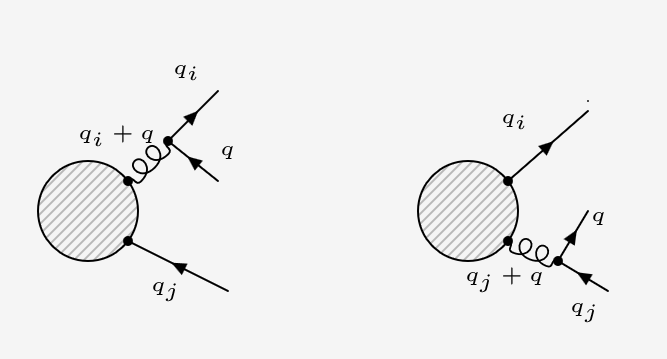
\includegraphics[width=0.85\textwidth]{images/QG/QGDiagrams.png}
\end{figure}

This case concerns a daughter quark from a parent gluon which splits into a quark-anti-quark pair. Here no singularity develops since daughter and parent can always be distinguished.\\
This is the reason why the calculation is not mentioned here, because the evaluation is analogous to the other parts considered so far.
\pagebreak
%
%\section{Quark loop}
%\begin{figure}[ht!]
%\centering
%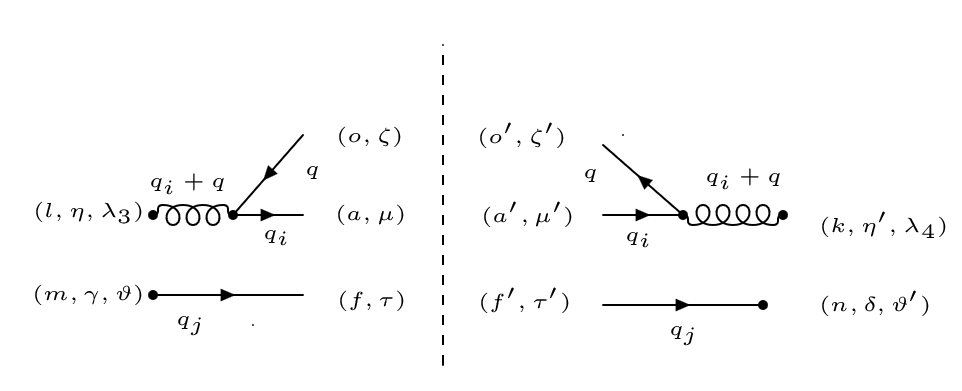
\includegraphics[scale=0.7]{images/QG/M1Squer.png}
%\end{figure}
%
%\begin{equation}
%\begin{split}
%|M_1|^2=[\frac{-i}{(q_i +k_1)^2}\not{q_i}(-ig_s {\gamma}^{\eta}\times{[T^l]_a}^o)\not{q}(ig_s {\gamma}^{{\eta}^{\prime}}\times{[T^k]_{o^{\prime}}}^{a^{\prime}})\frac{i}{(q_i +k_1)^2}][\not{q_k}]
%\end{split}
%\end{equation}
%
%
%\begin{equation}
%\begin{split}
%|M_1|^2=\frac{{g_s}^2 {[T^l]_a}^o {[T^k]_{o^{\prime}}}^{a^{\prime}}}{4(k_1 \cdot q_i)(k_1 \cdot q_i)}[ {k_1}_{\alpha} {q_i}_{\mu}\:(\gamma^{\mu}{\gamma}^{\eta}\gamma^{\alpha}\: {\gamma}^{{\eta}^{\prime}})][\not{q_k}]
%\end{split}
%\end{equation}
%
%
%\begin{equation}
%\begin{split}
%|M_1|^2=\frac{{g_s}^2 {[T^l]_a}^o {[T^k]_{o^{\prime}}}^{a^{\prime}}}{4(k_1 \cdot q_i)(k_1 \cdot q_i)}[{q_i}_{\mu}{k_1}_{\alpha}\:(2g^{{\eta}{\mu}}-{\gamma}^{\eta}\gamma^{\mu})\gamma_{\alpha}\: {\gamma}^{{\eta}^{\prime}}][\not{q_k}]
%\end{split}
%\end{equation}
%
%\begin{equation}
%\begin{split}
%|M_1|^2=\frac{{g_s}^2 {[T^l]_a}^o {[T^k]_{o^{\prime}}}^{a^{\prime}}}{4(k_1 \cdot q_i)(k_1 \cdot q_i)}[(2{q_i}^{\eta}\not{k_1}\:-{\gamma}^{\eta}\not{q_i}\not{k_1})\: {\gamma}^{{\eta}^{\prime}}][\not{q_k}]
%\end{split}
%\end{equation}
%
%\begin{equation}
%\begin{split}
%|M_1|^2=\frac{{g_s}^2 {[T^l]_a}^o {[T^k]_{o^{\prime}}}^{a^{\prime}}}{4(k_1 \cdot q_i)(k_1 \cdot q_i)}[(2{q_i}^{\eta}\not{k_1}\:-{\gamma}^{\eta}\not{q_i}\not{k_1})\: {g}^{{\eta}^{\prime} \eta} \gamma_{\eta}][\not{q_k}]
%\end{split}
%\end{equation}
%
%\begin{equation}
%\begin{split}
%|M_1|^2=\frac{{g_s}^2 {[T^l]_a}^o {[T^k]_{o^{\prime}}}^{a^{\prime}}}{4(k_1 \cdot q_i)(k_1 \cdot q_i)}(2{q_i}^{\eta}\not{k_1}\gamma_{\eta}\:-{\gamma}^{\eta}\not{q_i}\not{k_1}\gamma_{\eta})\: [{g}^{{\eta}^{\prime} \eta} ][\not{q_k}]
%\end{split}
%\end{equation}
%
%\begin{equation}
%\begin{split}
%|M_1|^2=\frac{{g_s}^2 {[T^l]_a}^o {[T^k]_{o^{\prime}}}^{a^{\prime}}}{4(k_1 \cdot q_i)(k_1 \cdot q_i)}(2\not{k_1}\not{q_i}\:-{q_i}_{\mu} {k_1}_{\alpha}{\gamma}^{\eta}{\gamma}^{\mu}{\gamma}^{\alpha}\gamma_{\eta})\: [{g}^{{\eta}^{\prime} \eta} ][\not{q_k}]
%\end{split}
%\end{equation}
%
%\begin{equation}
%\begin{split}
%|M_1|^2=\frac{{g_s}^2 {[T^l]_a}^o {[T^k]_{o^{\prime}}}^{a^{\prime}}}{4(k_1 \cdot q_i)(k_1 \cdot q_i)}(2\not{k_1}\not{q_i}\:-{q_i}_{\mu} {k_1}_{\alpha}(4g^{\alpha \mu}))\: [{g}^{{\eta}^{\prime} \eta} ][\not{q_k}]
%\end{split}
%\end{equation}
%
%\begin{equation}
%\begin{split}
%|M_1|^2=\frac{{g_s}^2 {[T^l]_a}^o {[T^k]_{o^{\prime}}}^{a^{\prime}}}{4(k_1 \cdot q_i)(k_1 \cdot q_i)}(2\not{k_1}\not{q_i}\:-4({q_i} \cdot {k_1}))\: [{g}^{{\eta}^{\prime} \eta} ][\not{q_k}]
%\end{split}
%\end{equation}
%
%\begin{equation}
%\begin{split}
%&|M_1|^2=\frac{{g_s}^2 {[T^l]_a}^o {[T^k]_{o^{\prime}}}^{a^{\prime}}}{4y^2\:(p_i\cdot Q)(p_i\cdot Q) }\\&
%(2(\zeta_1 \not{p_i} + \lambda_1\not{Q} + \sqrt{y\alpha_1\beta_1}\not{n}_{\bot,1} )( \zeta_q\not{p_i} + \lambda_q\not{Q} - \sqrt{y\alpha_1\beta_1}\not{n}_{\bot,l})-4y\:(p_i\cdot Q ))\: [{g}^{{\eta}^{\prime} \eta} ][\not{q_k}]
%\end{split}
%\end{equation}
%
%\begin{equation}
%\begin{split}
%&|M_1|^2=\frac{{g_s}^2 {[T^l]_a}^o {[T^k]_{o^{\prime}}}^{a^{\prime}}}{4y^2\:(p_i\cdot Q)(p_i\cdot Q) }\\&
%(2\zeta_1\lambda_q \not{p_i}\not{Q} +2\lambda_1\zeta_q\not{Q}\not{p_i} - 2{y\alpha_1\beta_1}{{n}_{\bot,1}}^2-4y\:(p_i\cdot Q ))\: [{g}^{{\eta}^{\prime} \eta} ][\not{q_k}]
%\end{split}
%\end{equation}
%
%\begin{equation}
%\begin{split}
%&|M_1|^2=\frac{{g_s}^2 {[T^l]_a}^o {[T^k]_{o^{\prime}}}^{a^{\prime}}}{4y^2\:(p_i\cdot Q)(p_i\cdot Q) }\\&
%(2y\alpha_1^2 \not{p_i}\not{Q} +2y\beta_1^2\not{Q}\not{p_i} - 2{y\alpha_1\beta_1}{{n}_{\bot,1}}^2-4y\:(p_i\cdot Q ))\: [{g}^{{\eta}^{\prime} \eta} ][\not{q_k}]
%\end{split}
%\end{equation}
%
%\pagebreak

%\section{Spectator Quark loop}
%\begin{figure}[ht!]
%\centering
%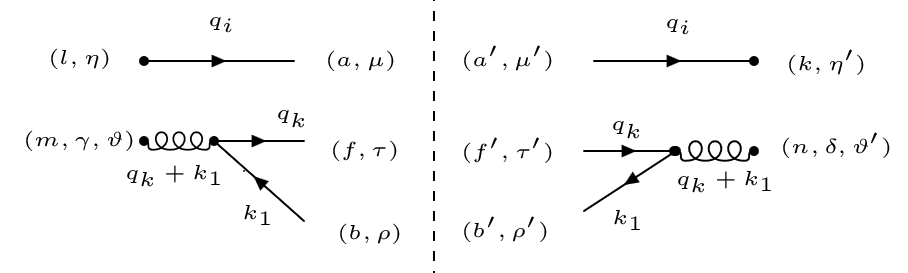
\includegraphics[scale=0.7]{images/QG/M2Squer.png}
%\end{figure}
%
%\begin{equation}
%\begin{split}
%|M_2|^2=\frac{{g_s}^2 {[T^m]_f}^b {[T^n]_{f}}^{b}}{4(k_1 \cdot q_k)(k_1\cdot q_k)}[\not{q_k}{\gamma}^{\gamma}\not{k_1}\:\: {\gamma}^{{\delta}}][\not{q_i}]
%\end{split}
%\end{equation}
%
%\pagebreak
%
%\section{Interference term}
%\begin{figure}[ht!]
%\centering
%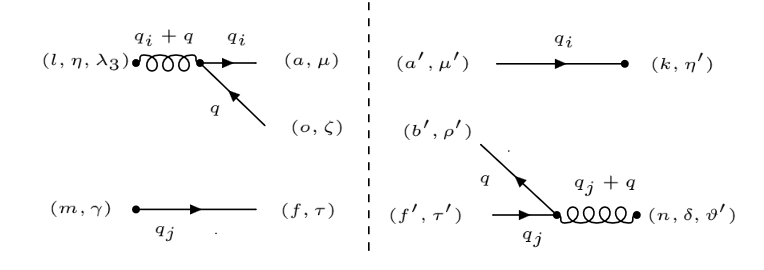
\includegraphics[scale=0.7]{images/QG/M1M2Dagger.png}
%\end{figure}
%
%
%\begin{equation}
%\begin{split}
%M_1\: {M_2}^{\dagger}=\frac{{g_s}^2 {[T^l]_a}^o {[T^n]_{f}}^{o}}{4(k_1 \cdot q_i)(k_1 \cdot q_k)}[\not{q_i}{\gamma}^{\eta}\not{k_1}][\: {\gamma}^{{\delta}}\not{q_k}]
%\end{split}
%\end{equation}
%
%\begin{equation}
%\begin{split}
%M_1\: {M_2}^{\dagger}=\frac{{g_s}^2 {[T^l]_a}^o {[T^n]_{f}}^{o}}{4(k_1\cdot q_i)(k_1 \cdot q_k)}[2\not{q_i}{k_1}^{\eta}-\not{q_i}\not{k_1}{\gamma}^{{\eta}}][\: g^{\delta \eta}{\gamma}_{{\eta}}\not{q_k}]
%\end{split}
%\end{equation}
%
%\begin{equation}
%\begin{split}
%M_1\: {M_2}^{\dagger}=\frac{{g_s}^2 {[T^l]_a}^o {[T^n]_{f}}^{o}}{4(k_1\cdot q_i)(k_1 \cdot q_k)}[2\not{q_i}\not{k_1}-d\not{q_i}\not{k_1}][\: g^{\delta \eta}][\not{q_k}]
%\end{split}
%\end{equation}
%
%\begin{equation}
%\begin{split}
%&M_1\: {M_2}^{\dagger}=(2-d)\frac{{g_s}^2 {[T^l]_a}^o {[T^n]_{f}}^{o}}{4y(1-\beta_1) (1-y)\:(p_i \cdot p_k)(p_i \cdot Q) }\\
%&[((\beta_1 -\alpha_1 y(\frac{Q^2}{2p_i \cdot Q}))\not{p_i} + y\alpha_1\not{Q} - \sqrt{y\alpha_1\beta_1}\not{n}_{\bot,1})\\&((\alpha_1 -y\beta_1(\frac{Q^2}{2p_i \cdot Q})) \not{p_i} + y\beta_1\not{Q} + \sqrt{y\alpha_1\beta_1}\not{n}_{\bot,1})][\: g^{\delta \eta}][\not{q_k}]
%\end{split}
%\end{equation}
%
%\begin{equation}
%\begin{split}
%&M_1\: {M_2}^{\dagger}=(2-d)\frac{{g_s}^2 {[T^l]_a}^o {[T^n]_{f}}^{o}}{4y(1-\beta_1) (1-y)\:(p_i \cdot p_k)(p_i \cdot Q) }\\
%&[\beta_1 \not{p_i}((\alpha_1 -y\beta_1(\frac{Q^2}{2p_i \cdot Q})) \not{p_i} + y\beta_1\not{Q}) ][\: g^{\delta \eta}][\not{q_k}]
%\end{split}
%\end{equation}
%
%\begin{equation}
%\begin{split}
%&M_1\: {M_2}^{\dagger}=(2-d)\frac{{g_s}^2 {[T^l]_a}^o {[T^n]_{f}}^{o}}{4y(1-\beta_1) (1-y)\:(p_i \cdot p_k)(p_i \cdot Q) }[y\beta_1^2 \not{p_i}\not{Q}) ][\: g^{\delta \eta}][\not{q_k}]
%\end{split}
%\end{equation}
%
%\section{$|M^{2}|$}
%
%\begin{equation}
%\begin{split}
%&|M|^{2}=|{M}_2|^{2}+|{M}_1|^{2}+2RE(M_1{M_2}^{\dagger})\\
%\end{split}
%\end{equation}